% Chapter Template

\chapter{Introducción general} % Main chapter title

\label{INTROGEN} % Change X to a consecutive number; for referencing this chapter elsewhere, use \ref{ChapterX}

%----------------------------------------------------------------------------------------
%	SECTION 1
%----------------------------------------------------------------------------------------

La conservación de la biodiversidad es un asunto del máximo interés teórico y práctico. Si en el pasado los esfuerzos se concentraron en la preservación de especies concretas, en la actualidad se comprende la importancia de proteger el sistema completo. Éste lo forman las especies y sus relaciones, tanto entre ellas como con el entorno. La Ecología se centra en el estudio de estas interacciones. Al igual que en otras ramas de la Biología, la clasificación de los fenómenos es un elemento central en el método de la ciencia ecológica. Así, las relaciones entre especies se denominan \textit{bióticas} mientras que las que mantienen con el entorno inanimado se llaman \textit{abióticas}. Toda la gama de las interacciones bióticas puede sistematizarse en unas pocas categorías. En la \textit{depredación} los individuos de una de las especies se benefician mientras que los de la otra resultan perjudicados, como en el \textit{parasitismo}. En la relación de \textit{competencia} los individuos, ya sean o no de la misma especie, disputan un mismo recurso. Estos tres tipos de interacción se caracterizan por la realimentación negativa, al actuar en sentidos opuestos sobre las dos especies. 

Si una de las especies obtiene beneficio pero la relación es neutral para la otra se habla de \textit{comensalismo}. Finalmente, si la relación es positiva para ambas especies, se trata de \textit{mutualismo}. En Ecología se contemplan estas relaciones desde un punto de vista funcional y mecanicista \cite{rockwood2006introduction}, atendiendo sobre todo a los flujos de intercambio de materia, energía o servicios.

El conjunto de interacciones crea sistemas de gran complejidad. La dinámica de las poblaciones, puede describirse utilizando modelos matemáticos. Además, en las últimas dos décadas, la ciencia de redes ha contribuido al conocimiento de las comunidades ecológicas aplicando sus propias técnicas de análisis. Estas descripciones, fundamentadas en modelos y propiedades topológicas, son fenomenológicas \cite{van2010ethical}.

Los distintos enfoques metodológicos en la investigación del mutualismo suponen a veces dificultades de comunicación, pero la colaboración resulta enriquecedora. Por ejemplo, la laboriosa toma de datos de los ecólogos de campo resulta imprescindible para que los modelos teóricos puedan contrastarse con la realidad, mientras que estos ayudan a explicar la estructura de las comunidades estudiadas \cite{ballantyne2015constructing}.

En esta tesis se plantean diversas contribuciones al estudio de las redes cooperativas que  caracterizan el \textit{mutualismo} desde el modelado matemático y la ciencia de redes, intentando no perder de vista su significado biológico.

\section{El mutualismo en ecología}

El término \textit{mutualismo} tuvo su origen en economía política a principios del XIX, relacionado con distintas concepciones utópicas. Fue el filósofo Pierre Joseph Proudhon el que hizo del mutualismo el eje de su teoría social y económica.

\enquote{\itshape [Mutualismo es] un sistema de equilibrio entre fuerzas libres, en el cual está cada una segura de gozar de los mismos derechos bajo la condición de llenar los mismos deberes, y 
de obtener las mismas ventajas a cambio de los mismos servicios} \cite{proudhon1868capacite}.

La idea de beneficio compartido fue trasladada al campo de la biología por el parasitólogo belga Pierre-Joseph van Beneden \cite{boucher1982ecology}, que escribió:

\enquote{\itshape Al lado [de los parásitos y comensales] hay otros que se prestan mutuamente servicios [..]. Creemos que es más justo llamarles Mutualistas} \cite{van1878commensaux}.

El mutualismo puede adoptar varias formas e intensidades. La característica que lo diferencia del resto de relaciones ecológicas es la cooperación entre especies que intercambian servicios o bienes \cite{bronstein2001exploitation}.


%-----------------------------------
%	SUBSECTION 1
%-----------------------------------
\subsection{Tipos de mutualismo}
\label{TIPOS_DE_MUTUALISMO}
	
Las relaciones mutualistas pueden clasificarse según distintos criterios. Por el \textbf{tipo de convivencia} se diferencia el \textit{mutualismo de simbiosis} del \textit{mutualismo no simbiótico}. En el primero, las especies solo pueden convivir en una relación íntima, como las que se establece entre numerosos animales y su flora intestinal o entre determinados tipos de bacterias y virus \cite{moran2005players, thrall2007coevolution}. En el segundo no hay convivencia permanente.
	
Atendiendo a la \textbf{naturaleza del beneficio recibido}, puede ser de bienes o servicios. La polinización pertenece al primer tipo. Los animales (invertebrados en su mayoría, pero también pequeños pájaros y murciélagos) se alimentan de polen o néctar y actúan a cambio como vectores de fertilización de las plantas. La biología de la polinización es muy rica. En ocasiones, las ceras o aceites florales pueden servir para la construcción de nidos, y algunas especies de flores han desarrollado engaños para los insectos que no reciben en esa situación ningún bien a cambio \cite{rech2014biologia}.

\begin{figure}[h!]
\centering
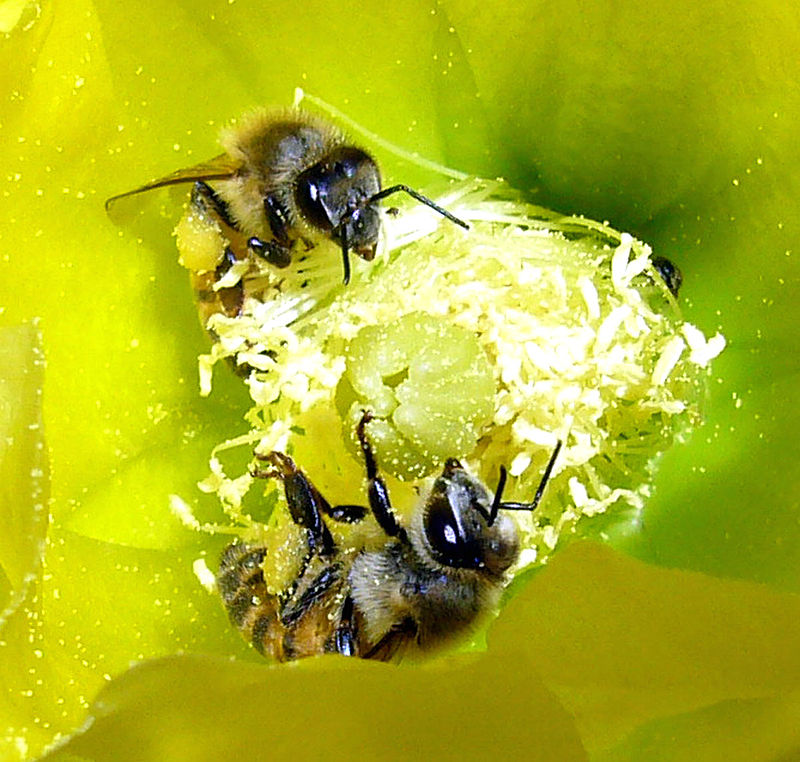
\includegraphics[scale=0.5]{Figures/INTRO_Pollination.jpg}
\caption{\textit{Apis mellifera} libando en una flor de \textit{Opuntia basilaris}, California (Estados Unidos). Fotografía de Jessie Eastland, \small{\texttt{CC BY-SA 3.0}}.}
\label{fig:INTRO_Pollination}
\end{figure}

Las comunidades de plantas y dispersores de semillas funcionan con el mismo esquema de intercambio de alimentación por servicio. Los frugívoros obtienen comida y en compensación reparten las semillas de la planta. Este tipo de mutualismo se registra sobre todo en los trópicos \cite{bascompte2007plant, estrada2012frugivores}.
	
Aunque menos comunes, también hay intercambios de recurso por recurso, como entre las bacterias del tipo \textit{Rhizobium} y las leguminosas a cuyas raíces se fijan. La bacteria proporciona compuestos nitrogenados a la planta y se alimenta de los azúcares que esta produce \cite{lindstrom2010biodiversity}.
	
Finalmente, el intercambio de servicio por servicio es la base de simbiosis como la de las anémonas con los peces y crustáceos que se han adaptado a vivir entre sus tentáculos venenosos. La anémona protege al huésped de los depredadores y a cambio este limpia sus parásitos \cite{mebs2009chemical}.

Otra distinción se basa en la \textbf{importancia vital para los actores}. En el \textit{mutualismo obligatorio} cada especie requiere del concurso de la otra para subsistir. Se suelen citar los ejemplos de la yuca y sus polillas (\textit{Prodixidae}) o el ya citado de la anémona, aunque hay dudas de que sean absolutamente obligatorios \cite{briand1982phylogenetic, addicott1995cheating}. Está muy asociado a una gran especialización y coevolución de los mutualistas. En el \textit{mutualismo facultativo}, la relación no tiene ese carácter esencial. Es el más común en las comunidades de plantas y polinizadores \cite{geib2012tracing}.

Una última distinción se basa en la \textbf{recepción directa o indirecta del beneficio}. El \textit{mutualismo directo} es el más común, pero a veces interviene una tercera especie que
intermedia entre las dos. Boucher, James y Keeler exponen diversos ejemplos en su artículo \cite{boucher1982ecology}. Desde un punto de vista de teoría de redes este \textit{mutualismo directo} se modela como dos enlaces unidireccionales entre ambas especies, en general con pesos diferentes en cada sentido.


\begin{figure}[h!]
\centering
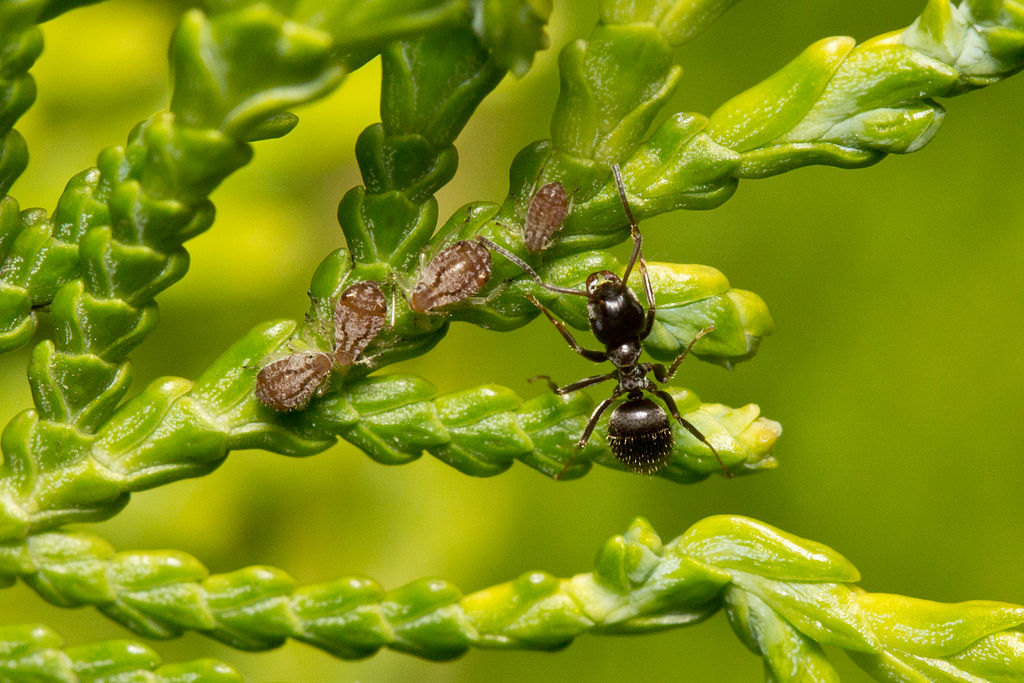
\includegraphics[scale=1]{Figures/INTRO_Lasius_niger_y_Cinara_tujafilina_en_Thuja_occidentalis.jpg}
\caption{\textit{Lasius niger} cuidando de varios ejemplares de \textit{Cinara tujafilina} sobre hojas de la conífera Tuya del Canadá \textit{Thuja occidentalis}. Fotografía de Carlos Delgado, \small{\texttt{CC BY-SA 3.0}}.}
\label{fig:INTRO_Lasius_niger_y_Cinara_tujafilina_en_Thuja_occidentalis}
\end{figure}

Los insectos sociales han desarrollado formas de mutualismo muy elaboradas. En la relación entre hormigas y áfidos se intercambia un servicio (protección) por alimento (ligamaza) \cite{volkl1999ant}. Bajo determinadas circunstancias la relación se transforma en depredación, las hormigas devoran a los áfidos, con una forma de explotación muy similar a la que se estableció en el Neolítico entre el ser humano y animales domesticados como la oveja. Otras especies cultivan hongos en sus hormigueros \cite{mueller2001origin}, en un comportamiento que también se asemeja a la relación de mutualismo que supone la agricultura.

A veces, las relaciones son complejas. Las hormigas actúan como protectoras de las acacias de las que reciben alimento y también protección contra depredadores con las púas de estos árboles \cite{raine2002spatial}. Las asociaciones entre \textit{mirmecofitas} y hormigas son muy especializadas y de naturaleza simbiótica \cite{djieto2004symbiotic}.También se documenta un tipo de mutualismo indirecto entre robles y hormigas, mediado por áfidos. La abundancia de estos no daña al árbol y beneficia a las hormigas, que a su vez, actúan como defensa frente a insectos que deterioran las bellotas \cite{ito1991indirect}.


%----------------------------------------------------------------------------------------
%	SECTION 2
%----------------------------------------------------------------------------------------

\section{Redes en ecología}

Una red es un conjunto de entidades entre las que se establecen relaciones. Representando las primeras como nodos y las segundas como enlaces, 
se construye un grafo, un modelo abstracto muy versátil. La estructura depende solo de su conformación, no de la realidad que representa. La ciencia de redes es una disciplina de desarrollo reciente que estudia cualquier fenómeno al que pueda aplicarse este método de modelado. Utiliza técnicas propias de la teoría de grafos clásica, de la física estadística o de la sociometría y tiene un amplío espectro de aplicación: economía, biología, tecnología, historia, literatura... \cite{barabasi2002linked, newman2003structure, brandes2013network}

Las redes son ubicuas en biología \cite{mason2007graph, raymond2009network}. Aparecen en las rutas metabólicas, la expresión génica o en epidemiología, por citar tres ejemplos destacados. Las comunidades ecológicas son redes de interacciones y su estudio en calidad de tales es anterior al auge actual de la ciencia de redes. Los investigadores de las cadenas tróficas ("\textit{food webs}", fig. \ref{fig:INTRO_Chengjiang_and_Burgess_Shale_1}) fueron los que abrieron este camino \cite{pimm1982food,martinez1992constant}.

\begin{figure}[h!]
\centering
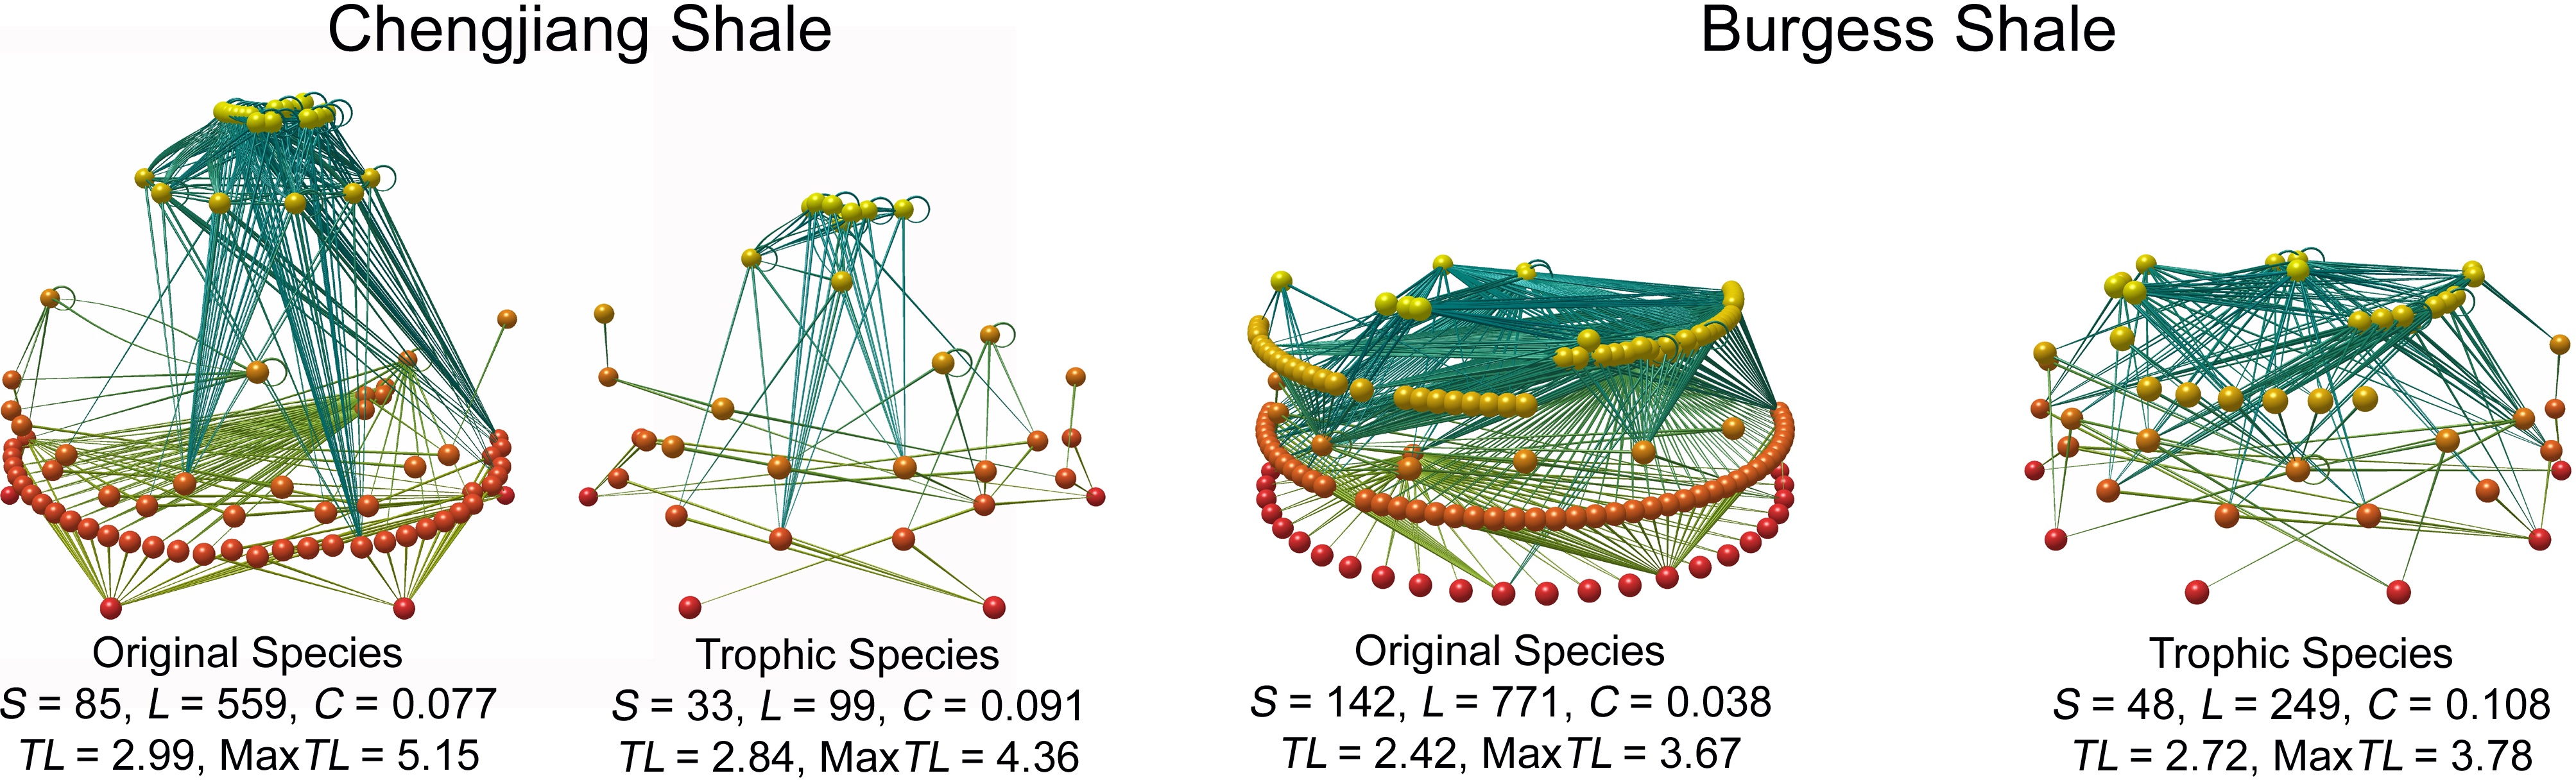
\includegraphics[scale=0.75]{Figures/INTRO_Chengjiang_and_Burgess_Shale_1.png}
\caption{Ejemplo de representación de cadenas tróficas como redes \cite{dunne2008compilation}. \small{\texttt{CC BY-SA 2.5}}.}
\label{fig:INTRO_Chengjiang_and_Burgess_Shale_1}
\end{figure}


\subsection{Redes mutualistas}

Las comunidades mutualistas se pueden modelar, en su forma más general, como redes bipartitas, dirigidas y pesadas. Son bipartitas porque existen dos clases de nodos y las relaciones solo pueden establecerse entre especies de clases distintas. Los enlaces modelan el beneficio que la especie $X$ de la clase $A$ aporta a la especie $Z$ de la clase $B$, por tanto son pesados \cite{barrat2004architecture}. La intensidad de este beneficio no es la misma que la que que recibe $X$ de $Z$, de manera que la red es dirigida. La figura \ref{fig:INTRO_bip_ficticia} muestra un diagrama bipartito de una comunidad mutualista. Para hacer más legibles los diagramas reales, la interacción entre dos especies se simplifica como un solo enlace no dirigido.

Una de las objeciones que pueden hacerse al modelado de las comunidades mutualistas como redes es su enfoque reduccionista. Tan solo se incluyen las interacciones positivas entre especies, pero como se ha explicado en el apartado \ref{TIPOS_DE_MUTUALISMO} la realidad puede ser mucho más rica. La red es una abstracción a la que podrían añadirse otros tipos de relación, posiblemente complicando el modelo hasta hacerlo inmanejable y mezclando los efectos del mutualismo con los de otros tipos de relación ecológica. En este punto conviene recordar la reflexión de George Box que abre la tesis. No hay modelos perfectos, pero algunos resultan útiles. 

\begin{figure}[h!]
\centering
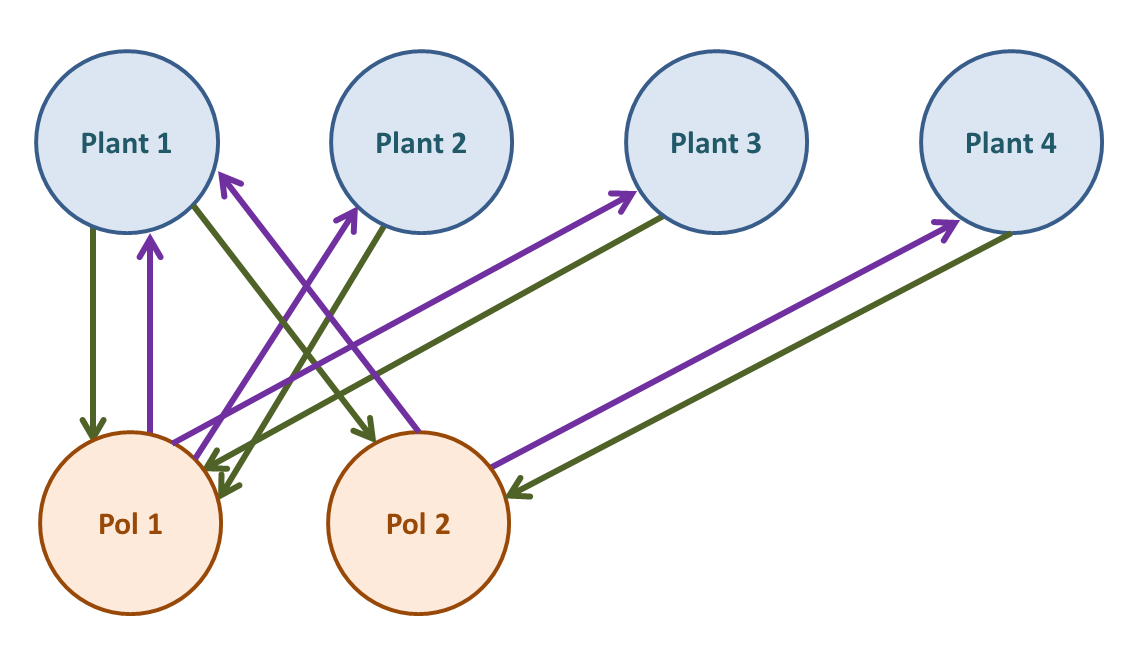
\includegraphics[scale=0.4]{Figures/INTRO_bip_ficticia.png}
\caption{Ejemplo de red mutualista con cuatro plantas y dos polinizadores}
\label{fig:INTRO_bip_ficticia}
\end{figure}

En su artículo seminal de 1987, Pedro Jordano aplicó de manera sistemática al mutualismo un enfoque de redes, utilizando las medidas que se habían empleado para las cadenas tróficas.

\enquote{\itshape Entender como se distribuyen el número y la fuerza de los enlaces entre los distintos pares de especies es básico para entender la evolución del mutualismo en un determinado contexto} \cite{jordano1987patterns}.

El análisis partía de la \textit{matriz de adyacencia}. Las especies de una clase se disponen como filas y las de la otra como columnas, si existe interacción la casilla de la matriz está rellena (figura \ref{fig:INTRO_M_PL_011a_matrix}). Jordano observó que el número de interacciones crece con el tamaño de la red, como cabía esperar. La \textit{conectancia}, entendida como la fracción del número de enlaces existentes entre todos los posibles presentaba una gran heterogeneidad. A partir de la publicación de este artículo, la literatura sobre redes mutualistas ha conocido un crecimiento sostenido y vive en la actualidad un periodo de florecimiento \cite{gu2015emerging}.

Además de la \textit{conectancia}, se han utilizado medidas habituales en el análisis genérico de redes. La \textit{distribución de grado} representa el número de enlaces por especie, y en las redes \textit{libres de escala} obedece a una ley de potencia. La mayoría de las comunidades mutualistas muestran una ley de potencia truncada \cite{jordano2003invariant}, lo que indica que no se forman de manera puramente aleatoria pero que tampoco se forman por \textit{conexión preferencial} \cite{barabasi1999emergence}. La explicación del mecanismo subyacente es aun objeto de debate pues no está claro si surge por restricciones de base biológica \cite{bascompte2007plant}, por pura estadística \cite{vazquez2005degree} o porque los datos disponibles no son suficientes y pueden tener sesgos de muestreo \cite{okuyama2008mutualistic, williams2011biology}. Por estos inconvenientes la distribución de grado no es la medida más útil en la caracterización del mutualismo.

Otras magnitudes de uso común como el \textit{clustering} o la \textit{distancia media} no son libres de escala, es decir, dependen del tamaño de la red \cite{olesen2006smallest}.

Además de la incertidumbre de los datos disponibles, la formación de las redes ecológicas, y en particular de las mutualistas, parece seguir distintas reglas que la de redes artificiales:

\enquote{\itshape El mecanismo de que los ricos serán más ricos está en contra de los principios ecológicos. Por ejemplo, cuantas más especies de frugívoros se alimenten de una misma especie de fruto, la competencia crecerá y será menos probable que otro frugívoro la incluya en su dieta y, por tanto, se alimentará de otras frutas.} \cite{montoya2006ecological}.

A pesar de todos estos obstáculos, el modelo de redes ha contribuido a avanzar en el estudio del mutualismo con el uso de magnitudes que describen de manera expresiva su estructura como la \textit{modularidad} y el \textit{anidamiento}.

\begin{figure}[h!]
\centering
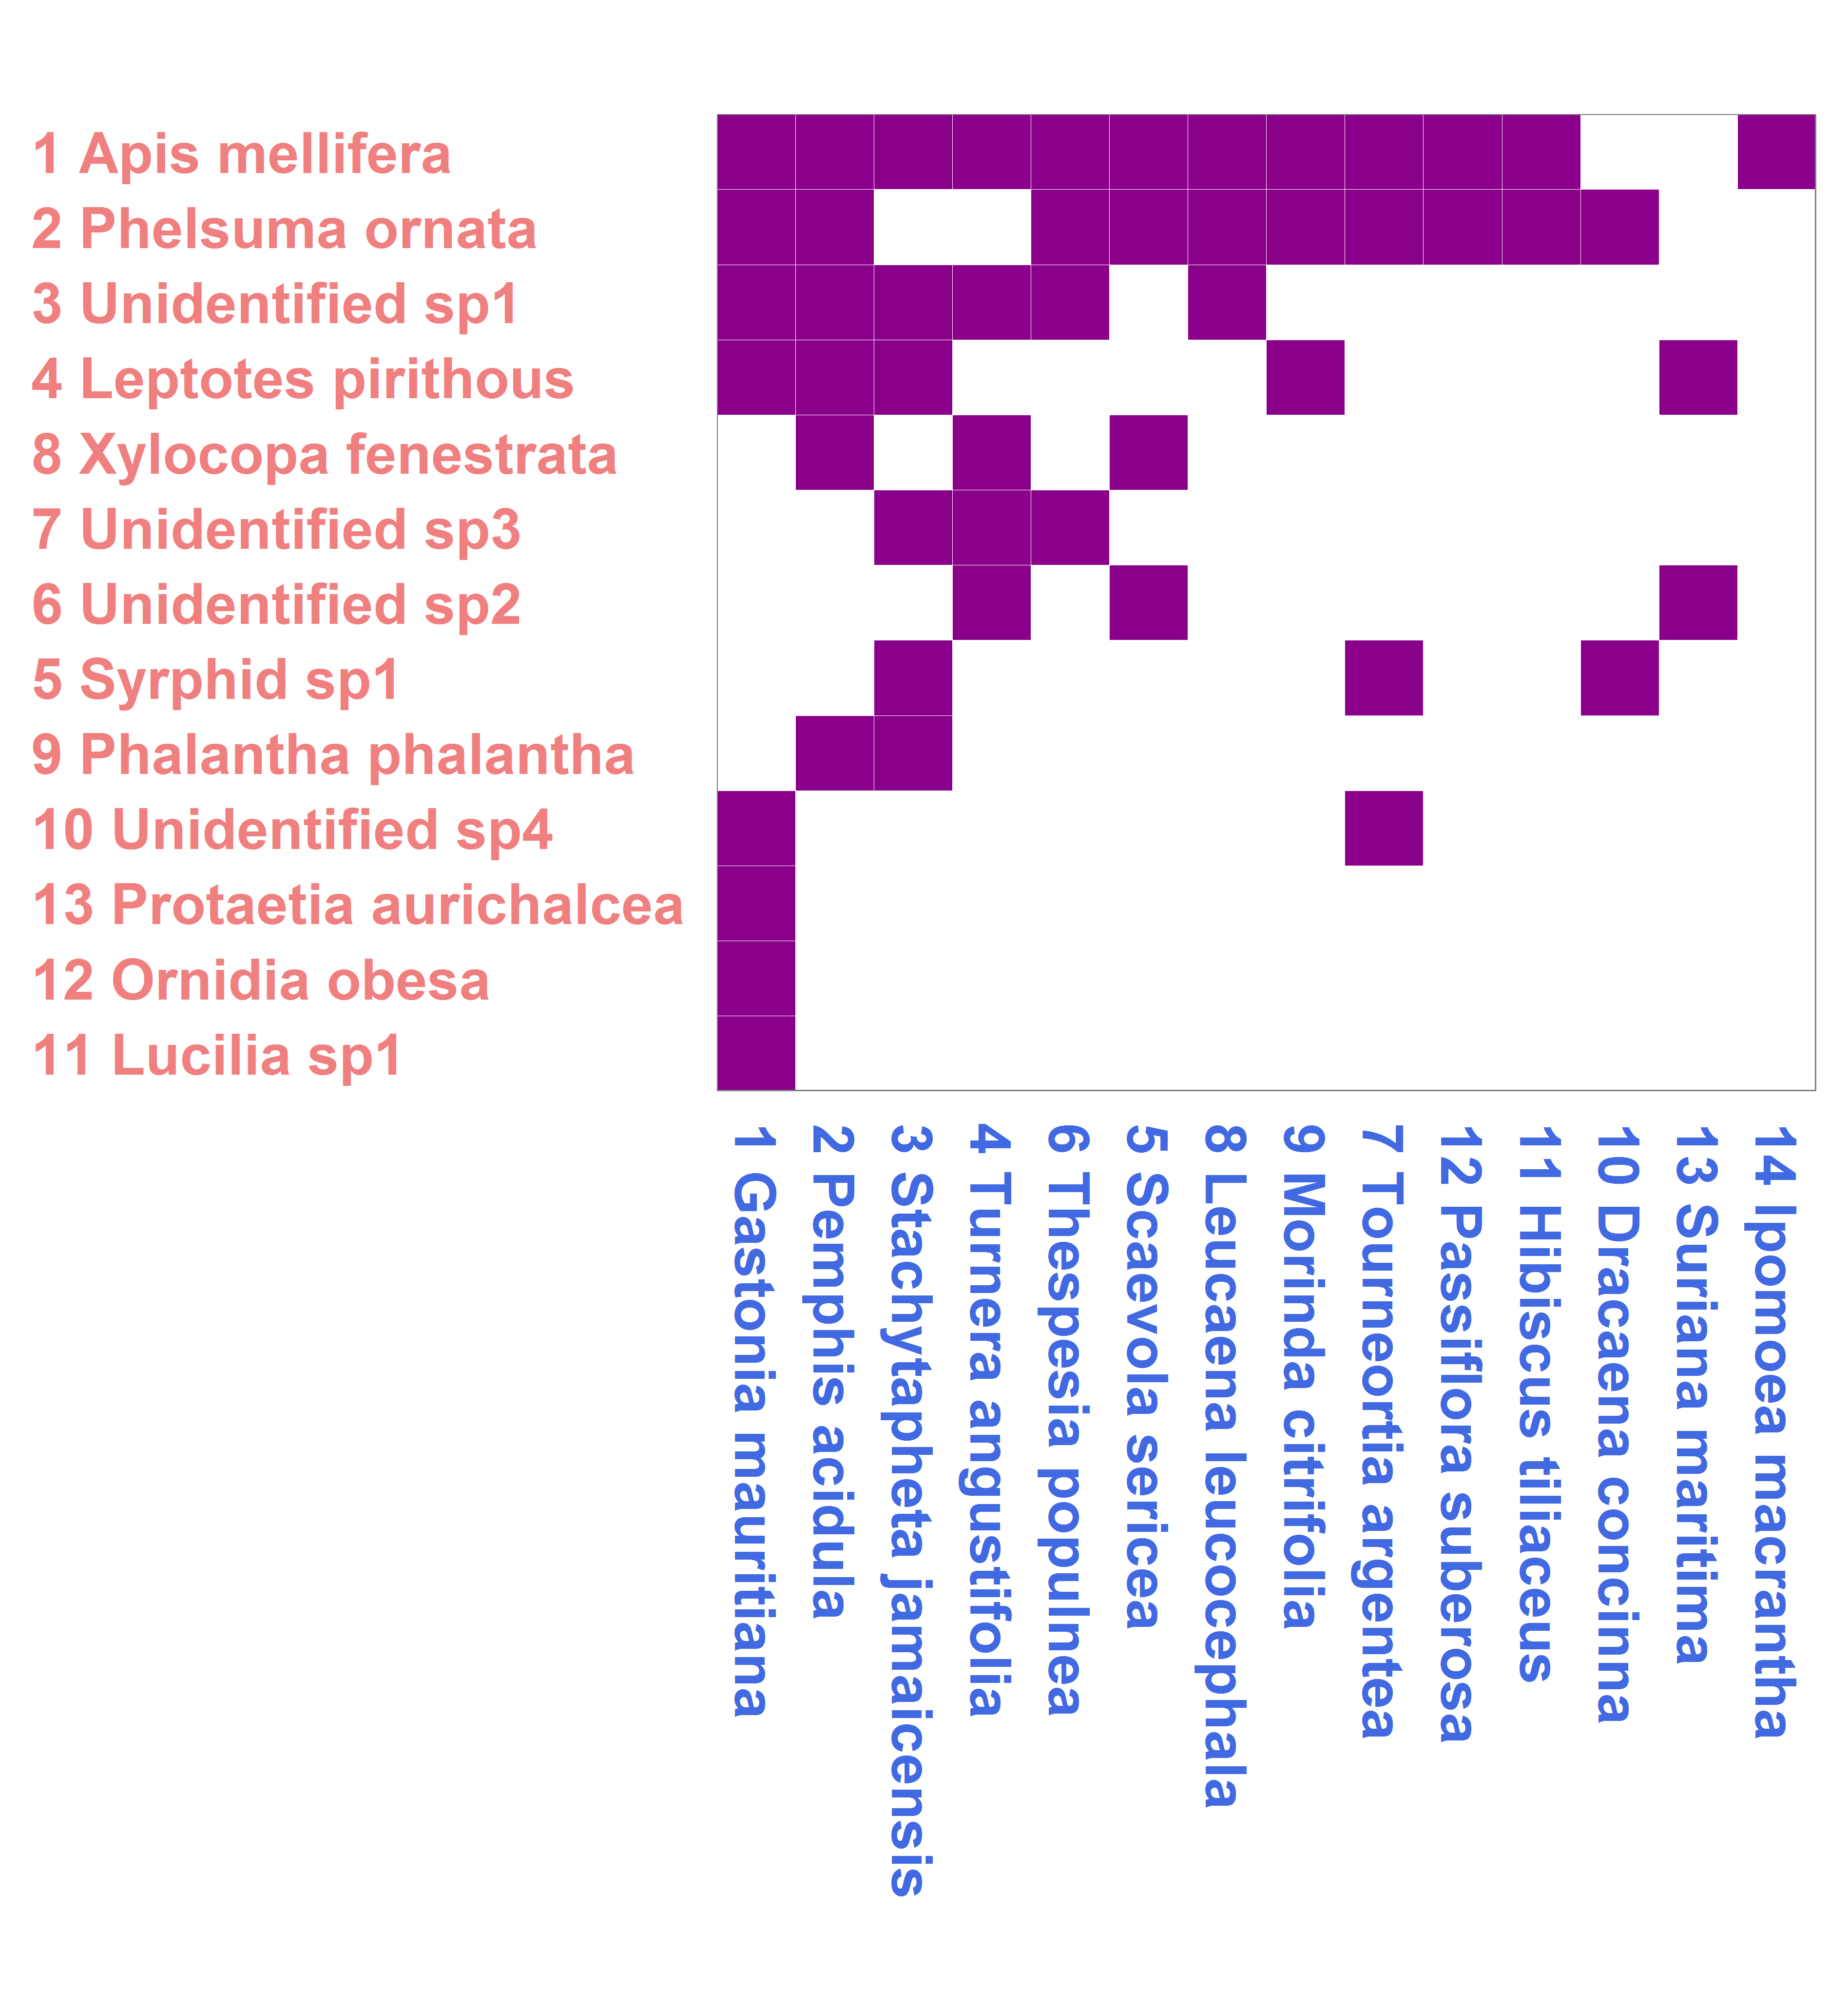
\includegraphics[scale=0.35]{Figures/INTRO_M_PL_011a_matrix.png}
\caption{Matriz de adyacencia de una red mutualista. Comunidad de plantas (en azul) y polinizadores (en salmón), Île aux Aigrettes (Mauricio) \cite{olesen2002invasion}.}
\label{fig:INTRO_M_PL_011a_matrix}
\end{figure}

De una forma intuitiva, la \textit{modularidad} expresa la existencia de conjuntos de nodos muy conectados dentro de una red con una densidad menor \cite{newman2006modularity}. Los módulos aparecen en las redes ecológicas por la existencia de complementariedad funcional entre las especies que los forman y aportan estabilidad frente a las extinciones en cascada \cite{olesen2007modularity, thebault2010stability, stouffer2011compartmentalization}.

El \textit{anidamiento} es una medida de organización jerárquica \cite{atmar1986nested} que se ha usado de manera habitual para caracterizar el mutualismo. Existe la evidencia empírica de que existe un núcleo de especies muy conectadas entre sí, a las que se denomina \textit{generalistas}. Por contra, las \textit{especialistas}, con uno o muy pocos enlaces interactuan con las generalistas pero raramente entre ellas \cite{bascompte2003nested, krishna2008neutral}. Esta disposición estructural es la que se cuantifica con el anidamiento.

Existe distintas medidas de anidamiento, que pueden usar la simplificación de tratar la matriz de adyacencia como binaria (\textit{nestedness temperature calculator} \cite{atmar1995nestedness}, $NODF$ \cite{almeida2008consistent}) o manejarla con sus pesos ($WINE$ \cite{galeano2009weighted}). Las conclusiones sobre el papel del anidamiento en la formación y estabilidad de las redes mutualistas dependen de la medida empleada, lo que hace que el debate académico sea intenso en la actualidad \cite{staniczenko2013ghost, strona2015new}. De lo que no cabe duda es del impulso que ha aportado este concepto a la investigación sobre las redes mutualistas.

\section{Dinámica de las comunidades mutualistas}

A pesar de su larga historia, hay aun muchos puntos abiertos en la investigación de la dinámica de poblaciones. Algunos de ellos fueron presentados en el 125 aniversario de la revista {\em Science} hace ya una década  \cite{kennedy2005,pennisi2005,stokstad2005}. Por ejemplo, los mecanismos que dan origen y mantienen la biodiversidad en un ecosistema son objeto de investigación desde campos diversos por la comunidad científica \cite{williams2000,dunne2002biodiversity,olesen2007modularity,allesina2008,bascompte2009,saavedra2009,bastolla2009,fortuna2010nestedness,encinas2012}.  

El antecedente más antiguo del estudio cuantitativo de las poblaciones se remonta a $1202$ cuando Leonardo Pisano (\textit{Fibonacci}), describió en su obra enciclopédica {\em Liber Abaci} la serie que sigue el crecimiento de una población de conejos \cite{sigler2002}. La teoría clásica de poblaciones, no obstante, se remonta a a $1798$ cuando Robert Malthus publicó {\em An Essay on the Principle of Population} \citep{malthus1798}. En dicha obra Malthus razonaba que el crecimiento de la población humana es proporcional al tamaño dado en un momento. Trasladándolo a una ecuación diferencial:
\begin{equation}
\frac{dN}{dt}=r_0\, N 
\label{eq:malthus}
\end{equation}
\noindent donde $N$ es el número de individuos y $r_0$ la {\em tasa intrínseca o vegetativa} de crecimiento de la polación, igual a la diferencia de las tasas de reproducción y defunciones cuando no hay migraciones.

El modelo malthusiano predice un crecimiento exponencial, así que si $r_0 > 0$ no tendría límite. En este modelo $r_0$ permanece constante a lo largo del proceso, sin tener en cuenta factores limitantes como la falta de alimentos o de espacio. En $1838$ Verhulst añadió un término adicional y llamó a su modelo modificado ecuación \emph{logística} \cite{verhulst1845}. La hipótesis de Verhulst es que la tasa de crecimiento debe reducirse conforme $N$ aumenta, hasta alcanzar un máximo. La forma matemática más simple de conseguirlo es haciendo que $r_0$ sea una función lineal de $N$: $ r_0 = r - \alpha N$, donde $r$ es la tasa intrínseca de crecimiento y $\alpha$ un coeficiente positivo de fricción que se interpreta como la competición entre los individuos de la misma especie por los recursos que permiten su crecimiento y supervivencia. El modelo $r/\alpha$ de Verhulst es:
\begin{equation}
\frac{dN}{dt}=r \, N \,  - \alpha  \, N^2 
\label{eq:primitiveverhulst}
\end{equation}
El término $\alpha$ actúa como un freno biológico, que sitúa al sistema en un punto de equilibrio cuando la población alcanza un valor $ K = r / \alpha$, comúnmente denominado \emph{capacidad de carga}.

Sin embargo, la ecuación logística se conoce mucho más en la forma que Raymond Pearl introdujo en un libro de biometría en $1930$ (véase una excelente reseña histórica en \cite{mallet2012struggle}). En esta formulación, que se impuso en los libros de texto y en la literatura científica, la capacidad de carga aparece como un parámetro explícito de la ecuación y por ello se conoce como la forma $r-K$:

\begin{equation}
\frac{dN}{dt}=r \, N \, \left(1-\frac{N}{K}\right)
\label{pearl}
\end{equation}

La solución de esta ecuación es una curva sigmoide que crece asintóticamente hacia $K$. La fórmula de Pearl tiene algunos inconvenientes matemáticos importantes \citep{kuno1991some,gabriel2005paradoxes}. El más notable es que predice un absurdo crecimiento si la tasa $r$ es negativa pero la población inicial está por encima de la capacidad de carga. Este problema fue señalado por Richard Levins y en consecuencia se denomina \textit{paradoja de Levins}. Es importante señalarlo, porque la mayoría de los modelos de mutualismo se han derivado de la logística en la formulación de Pearl y por tanto arrastran este inconveniente.

Para solucionar el problema Levins propuso que $r$ debía ser siempre no negativa. Gabriel \emph{et al.} encontraron una solución más elegante usando la formulación original de Verhulst \cite{gabriel2005paradoxes}. La condición para que el sistema alcance la estabilidad es que el coeficiente $\alpha$ sea siempre positivo y la capacidad de carga se redefine como:

\begin{equation}
K_{\infty}=\lim_{t\rightarrow\infty}N(t),\; N(0)>0
\end{equation}

\noindent y entonces
\begin{equation*}
K_{\infty}=\left\{
\begin{array}{ll}
  r / \alpha  = K, & \mathrm{si} \;\; r \geq 0, \\ 0  & \mathrm{si} \;\; r < 0 \\
  \end{array} \right.
\end{equation*}

Estos modelos primitivos de dinámica no incluían interacciones entre especies. Cuando varias de ellas comparten un mismo ecosistema aparece una compleja cadena de relaciones que puede modelarse como una red, como se mencionó en la sección precedente. En $1926$ Vito Volterra propuso un modelo de dos especies para explicar el comportamiento de algunos bancos de pesca en el Adriático \cite{volterra1926}. Las ecuaciones de Volterra describen las poblaciones de presa $N(t)$ y depredador $P(t)$ de la siguiente manera: 
\begin{align}
%\begin{split}
\displaystyle &\frac{dN}{dt}=N\, \left(a-b \,P\right) \nonumber\\
\displaystyle &\frac{dP}{dt}=P\, \left(c\, N-d\right) 
\label{myeq1}
%\end{split}
\end{align}
\noindent donde $a$, $b$, $c$ y $d$ son constantes positivas. En el modelo de Lotka-Volterra, como se conoce hoy, el crecimiento de la población de la presa está limitado por la población del depredador y viceversa. Este par de ecuaciones tiene una solución oscilatoria.

El mutualismo, probablemente porque es una interacción menos abundante en la naturaleza, ha recibido menos atención históricamente, también desde el punto de vista matemático. El primer modelo fue propuesto por Richard May \cite{may1981models}. Las ecuaciones de May son una modificación de la logística a la que se añade un tercer término que representa el beneficio mutualista. Es la misma idea que la del modelo Lotka-Volterra, pero con un inconveniente analítico, las interacciones son siempre positivas, de manera que no hay oscilaciones y sí la posibilidad de un crecimiento ilimitado. El modelo de May se formaliza como:
\begin{align}
\frac{dN_1}{dt}=r_1 \,N_1\,\left(1-\frac{N_1}{K_1}\right)+r_1\, N_1\,\beta_{12}\, \frac{N_2}{K_1} \nonumber \\ 
\frac{dN_2}{dt}=r_2\, N_2\, \left(1-\frac{N_2}{K_2}\right)+r_2\, N_2\, \beta_{21} \, \frac{N_1}{K_2} 
\label{myeq2}
\end{align}
\noindent donde $N_1(N_2)$ es la población de la especie $1(2)$; $r_1(r_2)$ es la tasa vegetativa de la población $1\, (2)$ y $K_1\, (K_2)$ la capacidad de carga. Este es el máximo que el entorno puede mantener en función de la disponibilidad de sustento y espacio. Por último, $\beta_{12}\,(\beta_{21})$ es el coeficiente que representa el beneficio mutualista para la especie $1\,(2)$ de su interacción con la $2\,(1)$.

El principal inconveniente del modelo de May es que conduce a crecimiento ilimitado. No obstante, ha servido de inspiración para todos sus sucesores que incorporan términos adicionales para solucionar este problema.

Ha habido diferentes estrategias de ataque. Wright propuso un modelo de dos especies con saturación como resultado de las restricciones del \textit{handling time}, $T_H$, que corresponde al tiempo necesario para procesar los recursos (comida) producidos por la relación mutualista \cite{wright1989}. Esto dio lugar a la familia de modelos conocida como \textit{tipo II}:
\begin{align}
\frac{dN_1}{dt}=r_1\, N_1\, - \alpha_1 \, N_1^2+ \frac{a\, b\, N_1\,N_2}{1+ a\, N_2\,T_H} \nonumber\\
\frac{dN_2}{dt}=r_2\, N_2\, - \alpha_2 N_2^2 + \frac{a\,b\,N_1\,N_2}{1+a\, N_1\, T_H}
\label{eq_typeII}
\end{align}
\noindent donde $a$ es la tasa efectiva de búsqueda y $b$ un coeficiente que tiene en cuenta los encuentros entre individuos de las especies $1$ y $2$. La dinámica del modelo depende en gran medida del afinado de los parámetros, pero para un rango limitado de ellos muestra tres puntos fijos. Uno estable, que corresponde con la destrucción completa, otro también estable en máximos de población y un \textit{saddle point} que separa las cuencas de atracción de los dos primeros. 

Usando un modelo tipo II, Bastolla demostró la importancia de la estructura de la red para minimizar la competencia entre especies y optimizar la biodiversidad \cite{bastolla2005,bastolla2009}. Los modelos de tipo II son, no obstante, difíciles de manejar analíticamente, debido a la forma en fracción del término mutualista. Hay otras alternativas recientes \cite{johnson2013} que proponen añadir términos adicionales al modelo tipo II, dificultando aun más el análisis.

\section{Propiedades estructurales del mutualismo}
\label{sec:prop_mutualismo}

Como ya se indicó, la investigación sobre la estructura del mutualismo heredó las herramientas conceptuales del análisis de las \textit{food webs}, entre ellas el uso de la \textit{conectancia}. Esta magnitud se define como la fracción de enlaces presentes de todos los posibles entre las especies de ambas clases. Resulta un índice global de utilidad limitada, pero sigue
usándose para la construcción de modelos nulos que veremos en este mismo capítulo. La distribución de grado es la traducción local de la conectancia, y es muy heterogénea en las redes mutualistas, con algunas especies mucho más conectadas de lo que cabría esperar por azar \cite{jordano2003invariant}.

Durante la última década el \textit{anidamiento} se ha considerado como la característica distintiva del mutualismo \cite{bascompte2003nested}, aunque en la actualidad esta afirmación está sujeta a revisión \cite{james2012disentangling, staniczenko2013ghost, jonhson2013factors, feng2014heterogeneity}. Este concepto tiene una definición clara en ecología, una comunidad es anidada si las especies encontradas en un ámbito geográfico reducido son un subconjunto de las existentes en un ámbito mayor más rico en recursos. Originalmente se aplicó al estudio de la distribución de la fauna en islas. La de una isla pequeña es un subconjunto de la que existe en tierra firme o en una isla mayor de las mismas características biogeográficas \cite{young1958zoogeography, atmar1986nested}.

Si las especies se ordenan por grado, la matriz de adyacencia de una comunidad con anidamiento fuerte muestra abundancia de interacciones entre las especies situadas en el vértice superior izquierdo. Allí se concentran las muy conectadas,
las de grado reducido aparecen conectadas con este núcleo y raramente entre ellas.

\begin{figure}[h!]
\centering
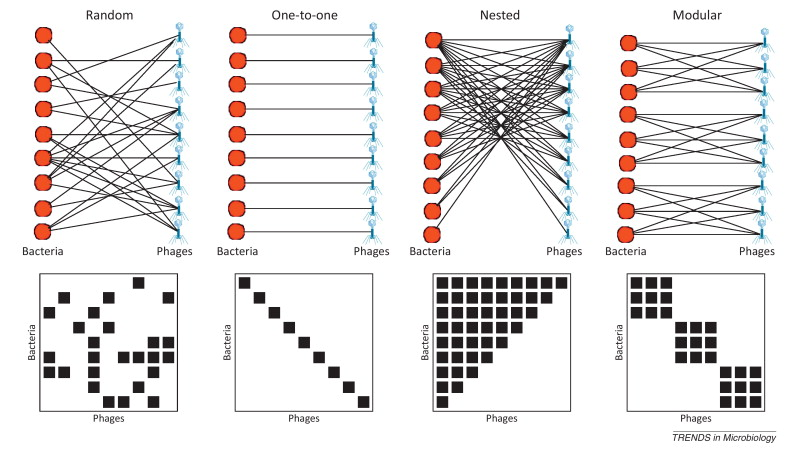
\includegraphics[scale=0.75]{Figures/ESTATICA_redes_ejemplos.png}
\caption{Explicación muy sencilla sobre la relación entre la forma de la matriz de adyacencia y la configuración de una red ecológica, en este caso de depredación \cite{weitz2013phage}. En la red perfectamente anidada las especies están ordenadas en orden decreciente de interacciones. Puede verse cómo se rellena la esquina superior izquierda de la matriz (generalistas) mientras que a medida que nos alejamos de esta las especies son cada vez más especialistas y solo interaccionan entre ellas. En la red modular aparecen grupos de especies con una fuerte cohesión que forman islas en la matriz de adyacencia. La realidad no es nunca ideal, y las redes mutualistas tienen anidamiento notable, pero también zonas de modularidad y relaciones que se parecen a las de una red aleatoria. Véanse las figuras \ref{fig:INTRO_M_PL_011a_matrix} y \ref{fig:VIS_matrix_SD_001}}
\label{fig:ESTATICA_redes_ejemplos}
\end{figure}


En las redes mutualistas se observa un grupo de especies generalistas con un alto número de conexiones y especialistas que se conectan con las generalistas pero apenas con otras especialistas. Esta organización, que tradicionalmente se ha caracterizado como anidamiento, parece proporcionar estabilidad estructural y maximizar las poblaciones de la comunidad \cite{memmott2004tolerance,bastolla2009,thebault2010stability,suweis2013emergence}. 

La medida del anidamiento es la más popular en el análisis del mutualismo, pero no está exenta de problemas. El principal es que existen distintos indicadores que no son equivalentes. No vamos a hacer una revisión de todos ellos, porque la producción en este terreno ha sido prolífica \cite{ulrich2009consumer}, pero mencionaremos los más destacados. 

Los basados en la \textit{temperatura} comparan la posición de los elementos de la matriz de adyacencia con la llamada isoclina de anidamiento perfecto. La curvatura de esta línea se define por la conectancia de la red. La temperatura se calcula con una función del número enlaces por debajo de la isoclina o los huecos por encima de ella y de la distancia a la que se encuentran de esta \cite{ulrich2007null}. El método más popular es el \textit{Nestedness Temperature Calculator} (NTC) de Atmar y Patterson \cite{atmar1995nestedness}.

Los métodos de tipo \textit{gap} se basan en un conteo del número de veces que habría que mover los enlaces de la matriz para conseguir un anidamiento perfecto. El primero en publicarse fue el llamado $BR$ \cite{brualdi1999nested}.

La tercera aproximación consiste en utilizar la definición original de anidamiento y medir la superposición (\textit{overlaping}). Se cuentan las interacciones por filas y columnas y se identifican las que son subconjuntos por similaridad. El primer índice en seguir este criterio fue el $HH$ \cite{hausdorf2003nestedness}. En los últimos años se han empleado mucho evoluciones de esta idea como $NODF$ (\textit{Node Overlap Decreasing Fill}) \cite{almeida2008consistent} y $PRN$ (\textit{Percentage Relativized Nestedness}) \cite{podani2012comparative}.

En los métodos descritos la matriz de adyacencia es binaria, o se trata como tal. Si se desea tener el cuenta el peso de los enlaces, en el
caso de que se disponga de datos, existen alternativas. $WNODF$ es una modificación de $NODF$ \cite{almeida2011straightforward}, mientras que $WINE$ se basa en la distancia Manhattan \cite{galeano2009weighted}. Por último, hay que citar el \textit{Radio Espectral} \cite{staniczenko2013ghost}. Este índice es el módulo del autovalor máximo de la matriz de adyacencia, y es válido tanto para matrices binarias como pesadas. 

\begin{figure}[h!]
\centering
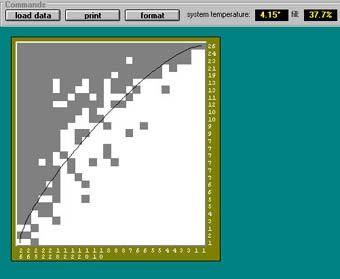
\includegraphics[scale=0.66]{Figures/ESTATICA_nested_subsets.jpg}
\caption{Interfaz de usuario del \textit{Nestedness Temperature Calculator}. Obsérvese la isoclina de anidamiento perfecto y las ocurrencias por debajo de ella \cite{atmar1995nestedness}.}
\label{fig:ESTATICA_nested_subsets}
\end{figure}

Otro indicador global que se emplea de forma habitual en la caracterización del mutualismo es la modularidad \cite{newman2004finding, olesen2007modularity}. De una forma intuitiva, los módulos son grupos de nodos fuertemente conectados entre sí dentro de una red con baja conectividad.
Al igual que sucede con el anidamiento, existen diferentes algoritmos para el cálculo de la modularidad. En mutualismo el
más usado es el de Barber para redes binarias \cite{barber2007modularity} y una versión reciente (\textit{QuanBiMo}) para redes pesadas \cite{dormann2014method}.

La relación entre modularidad y anidamiento en las redes mutualistas ha despertado el interés de la comunidad científica \cite{olesen2007modularity, dupont2009ecological}. Parecen comportarse como propiedades en cierto sentido antagónicas y por tanto como reguladoras de la estabilidad \cite{fortuna2010nestedness}. Por ejemplo, los módulos actúan como cortafuegos ante las extinciones en cascada \cite{saavedra2011strong} mientras que las redes muy anidadas son más vulnerables a este fenómeno \cite{lever2014sudden}. 

Ambas magnitudes se corresponden con propiedades globales de la red, pero no ofrecen medidas locales. No tiene sentido hablar de anidamiento o modularidad de una especie. Esta limitación supone un obstáculo en la práctica a la hora de definir políticas de conservación, porque no resultan útiles para predecir el comportamiento ante extinciones parciales. Desde un punto de vista analítico, también es deseable poder encontrar principios que funcionen tanto a escala global como a escala local. 
Además, la relación entre anidamiento, modularidad, abundancia de especies y establidad de la red es un tema de intenso debate académico \cite{fortuna2010nestedness, james2012disentangling, staniczenko2013ghost, feng2014heterogeneity}. Como resultado de todas estas consideraciones, la búsqueda de medidas alternativas, basadas en propiedades estadísticas o topológicas, es un campo de investigación muy activo \cite{podani2014new,chagnon2015characterizing,strona2015new}.

\section{Representaciones clásicas del mutualismo}

Las redes mutualistas son bipartitas y por ello no es extraño que el diagrama bipartito haya sido el más empleado en la literatura. En este 
gráfico los nodos se disponen en dos filas paralelas, ya sean horizontales o verticales, y se unen aquellos que comparten enlace. Cuando el tamaño
de la red es reducido, este diagrama tan simple funciona de manera satisfactoria.

\begin{figure}[h!]
\centering
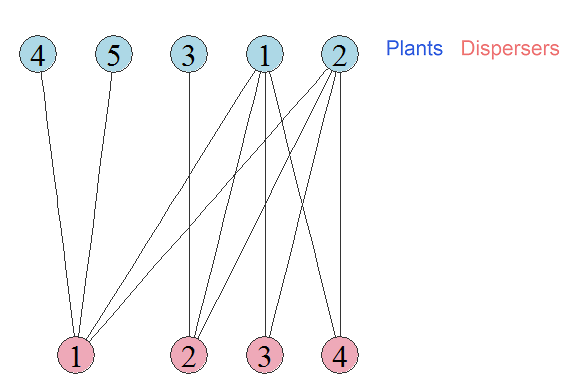
\includegraphics[scale=0.35]{Figures/VIS_SD_030_bipartita.png}
\caption{Diagrama bipartito de la red de dispersores de semillas que se usó como ejemplo de cálculo de las \textit{k magnitudes}. Véase la figura \ref{fig:ESTATICA_red_example}.}
\label{fig:Figures/VIS_SD_030_bipartita}
\end{figure}

En el ejemplo de la figura \ref{fig:Figures/VIS_SD_030_bipartita} puede distinguirse el núcleo de especies más conectadas (especies de plantas $1$ y $2$ y todos los polinizadores) y como las especialistas se conectan a él. Los enlaces se ven con claridad. No obstante, es difícil captar la estructura interna de la red. Sucede lo mismo en la representación de la figura \ref{fig:ESTATICA_red_example}. El diagrama bipartito es ideal para redes de afiliación, en las que el dato clave es la conexión entre los nodos de ambas clases, pero no permite apreciar las interacciones indirectas entre elementos de una misma clase que comparten enlace con un nodo de la contraria.

\begin{figure}[h!]
\centering
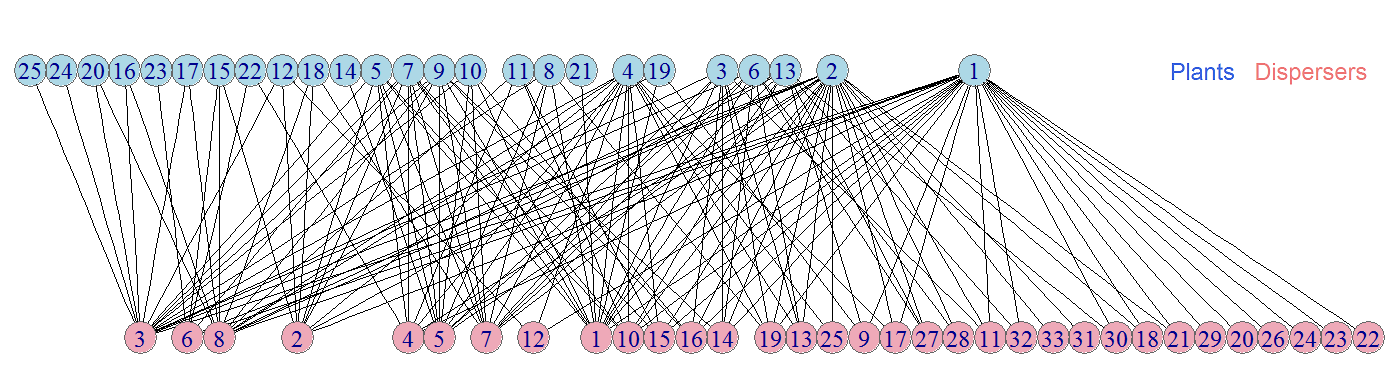
\includegraphics[scale=0.4]{Figures/VIS_bipartito_SD_020.png}
\caption{Red de dispersores en Nava Correhuelas, Sierra de Cazorla, España. Compilada por Pedro Jordano, no publicada.}
\label{fig:VIS_bipartito_SD_020}
\end{figure}

Cuando el número de especies supera unas pocas decenas, el diagrama bipartito se vuelve confuso. La red de la figura \ref{fig:VIS_bipartito_SD_020} tiene $58$ especies y $150$ enlaces, frente a $9$ especies y $11$ enlaces de la anterior. Es una red de dimensiones moderadas, pero es muy complicado seguir los detalles del gráfico. A pesar de ello, algunos autores consiguen resultados excelentes con redes de dimensiones similares a las de este segundo ejemplo, jugando con formas, colores y tamaños \cite{dakos2014critical}. Cuando se llega al centenar de especies, la zona central degenera en una mancha en la que es imposible distinguir los enlaces. Por este motivo, en la literatura sobre mutualismo no aparecen diagramas bipartitos de redes grandes. 

\begin{figure}[h!]
\centering
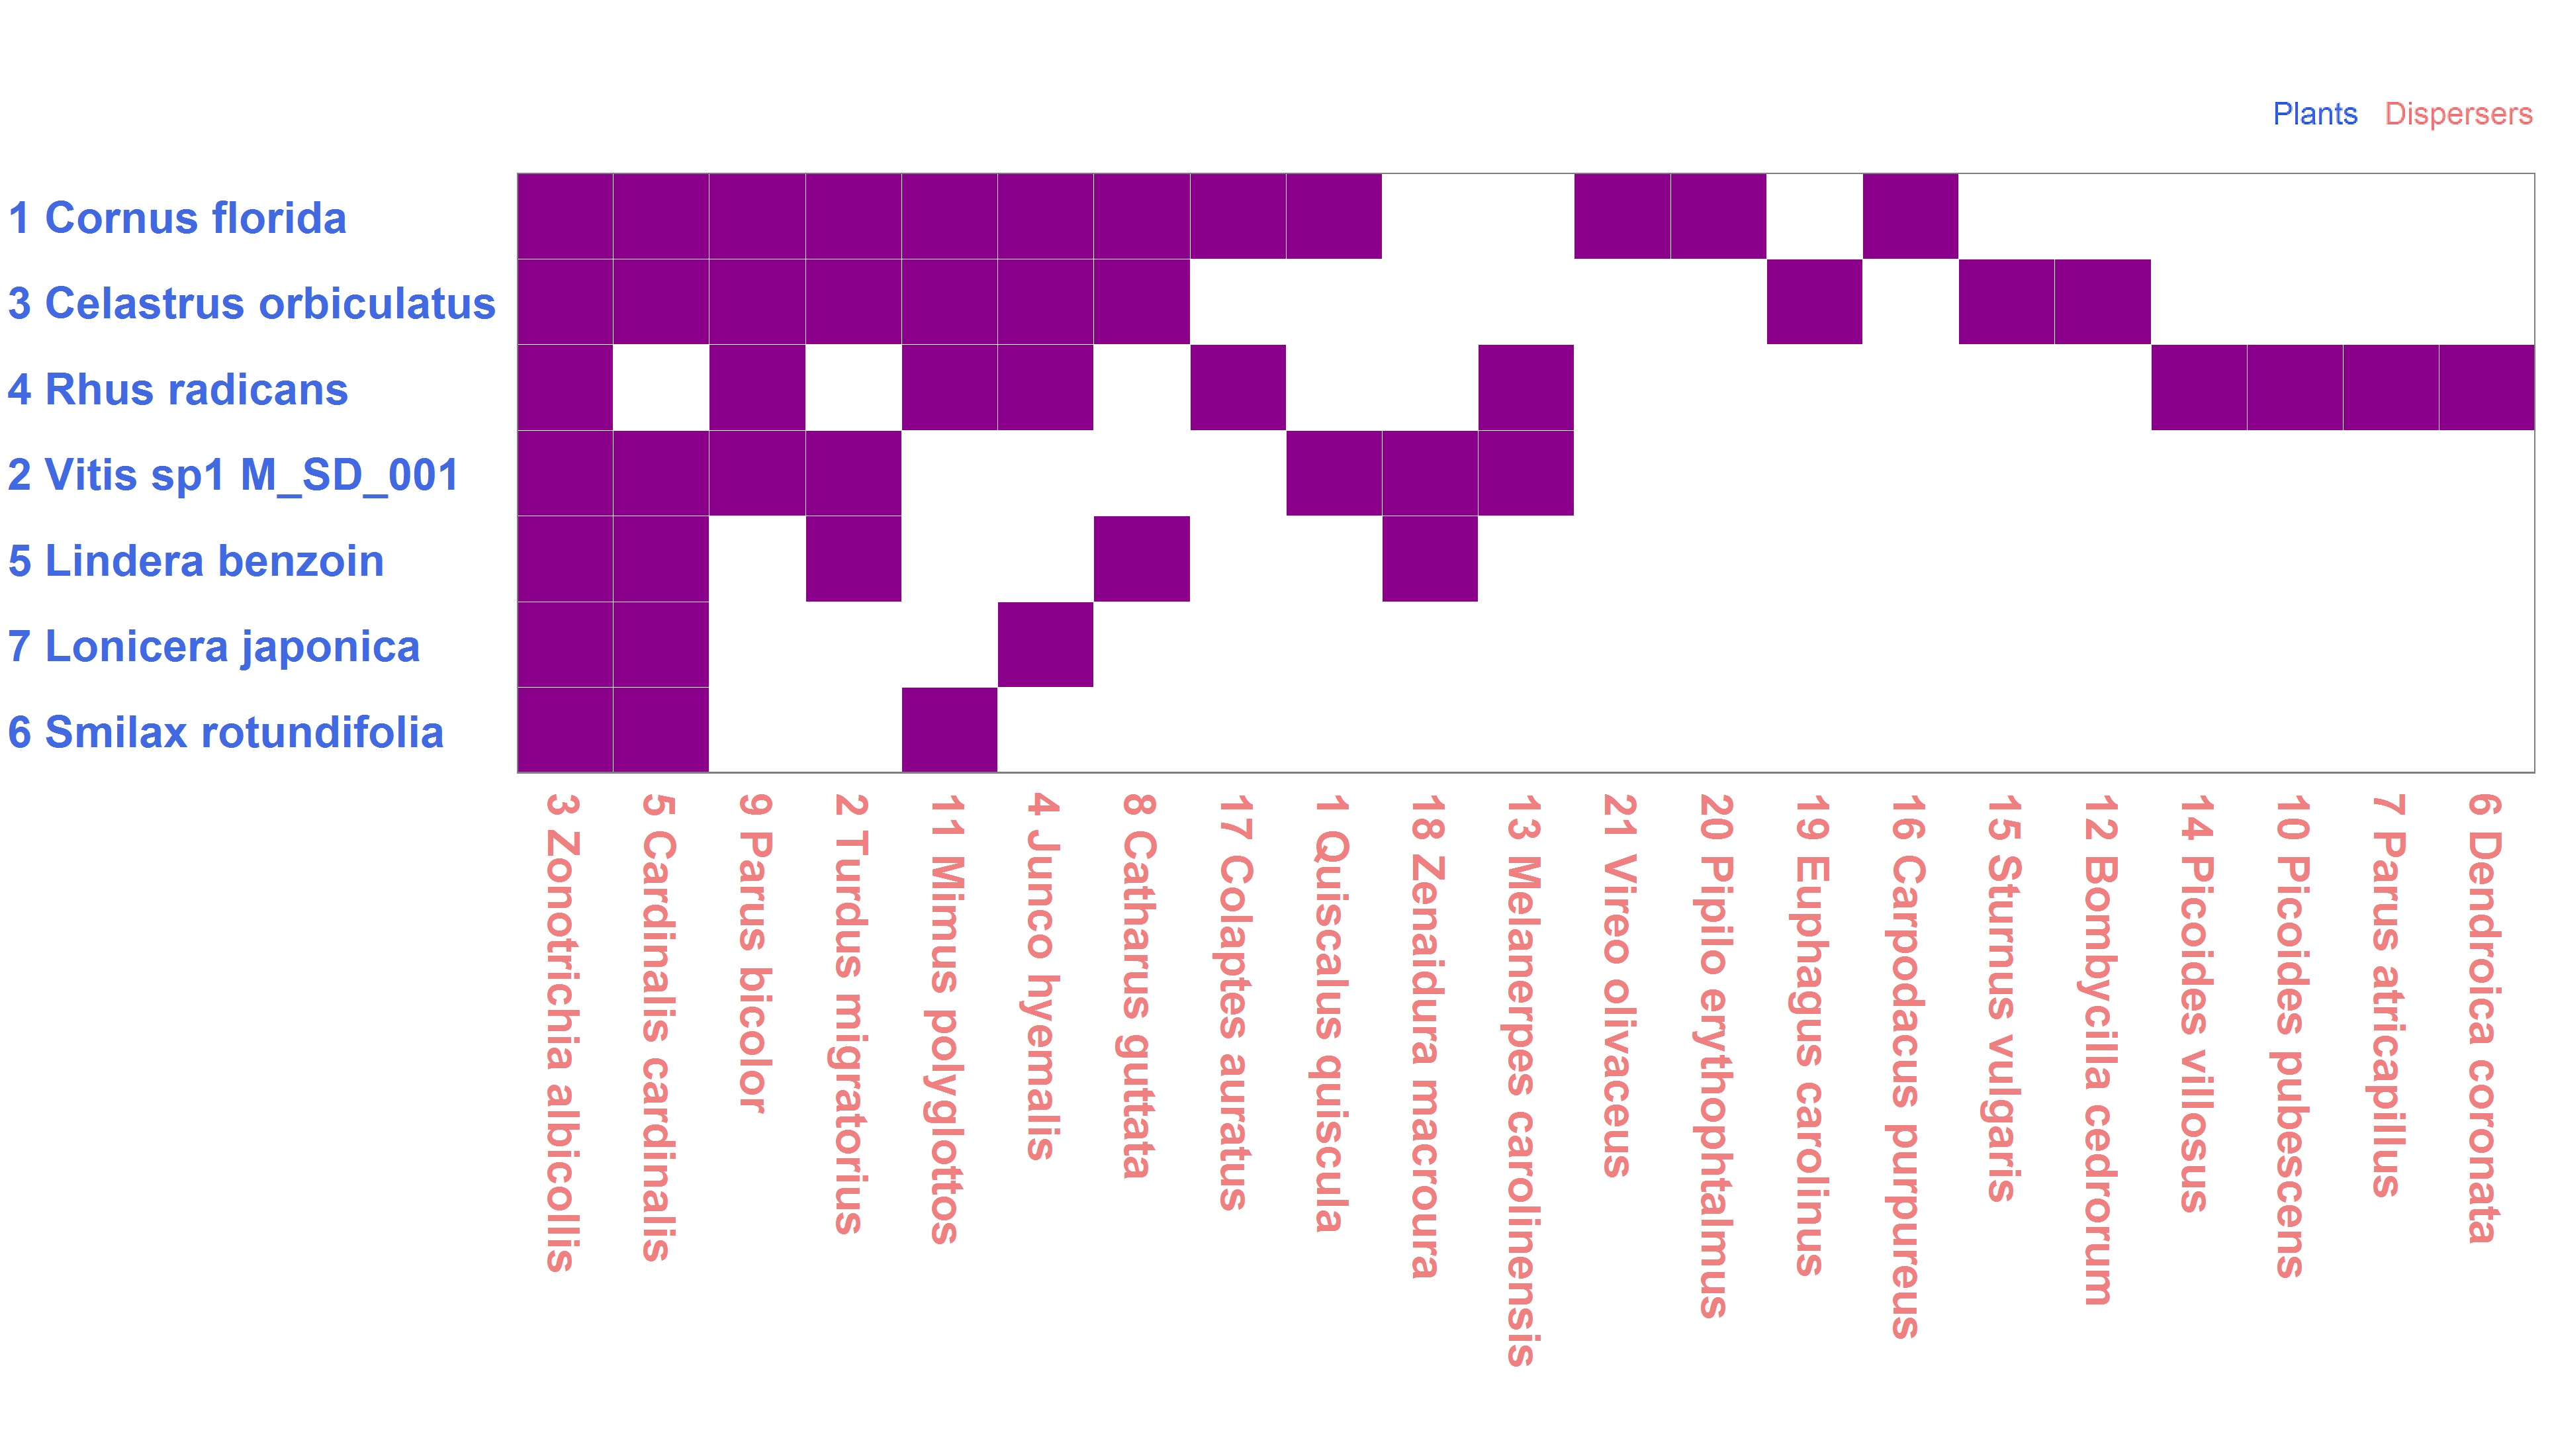
\includegraphics[scale=0.1]{Figures/VIS_matrix_SD_001.png}
\caption{Matriz de adyacencia de una red de dispersores en New Jersey \cite{baird1980selection}. Las casillas coloreadas indican la existencia de enlace.}
\label{fig:VIS_matrix_SD_001}
\end{figure}

La matriz de adyacencia ofrece una visión más rica si los nodos se ordenan de la forma adecuada. Colocando los más conectados en la parte superior izquierda, es fácil localizar el núcleo de especies generalistas. Para redes pequeñas, el resultado es muy bueno.
Por el contrario, esta representación gráfica se vuelve también muy confusa para redes grandes, como muestra la figura \ref{fig:VIS_matrix_PL_001}.

\begin{figure}[ht!]
\centering
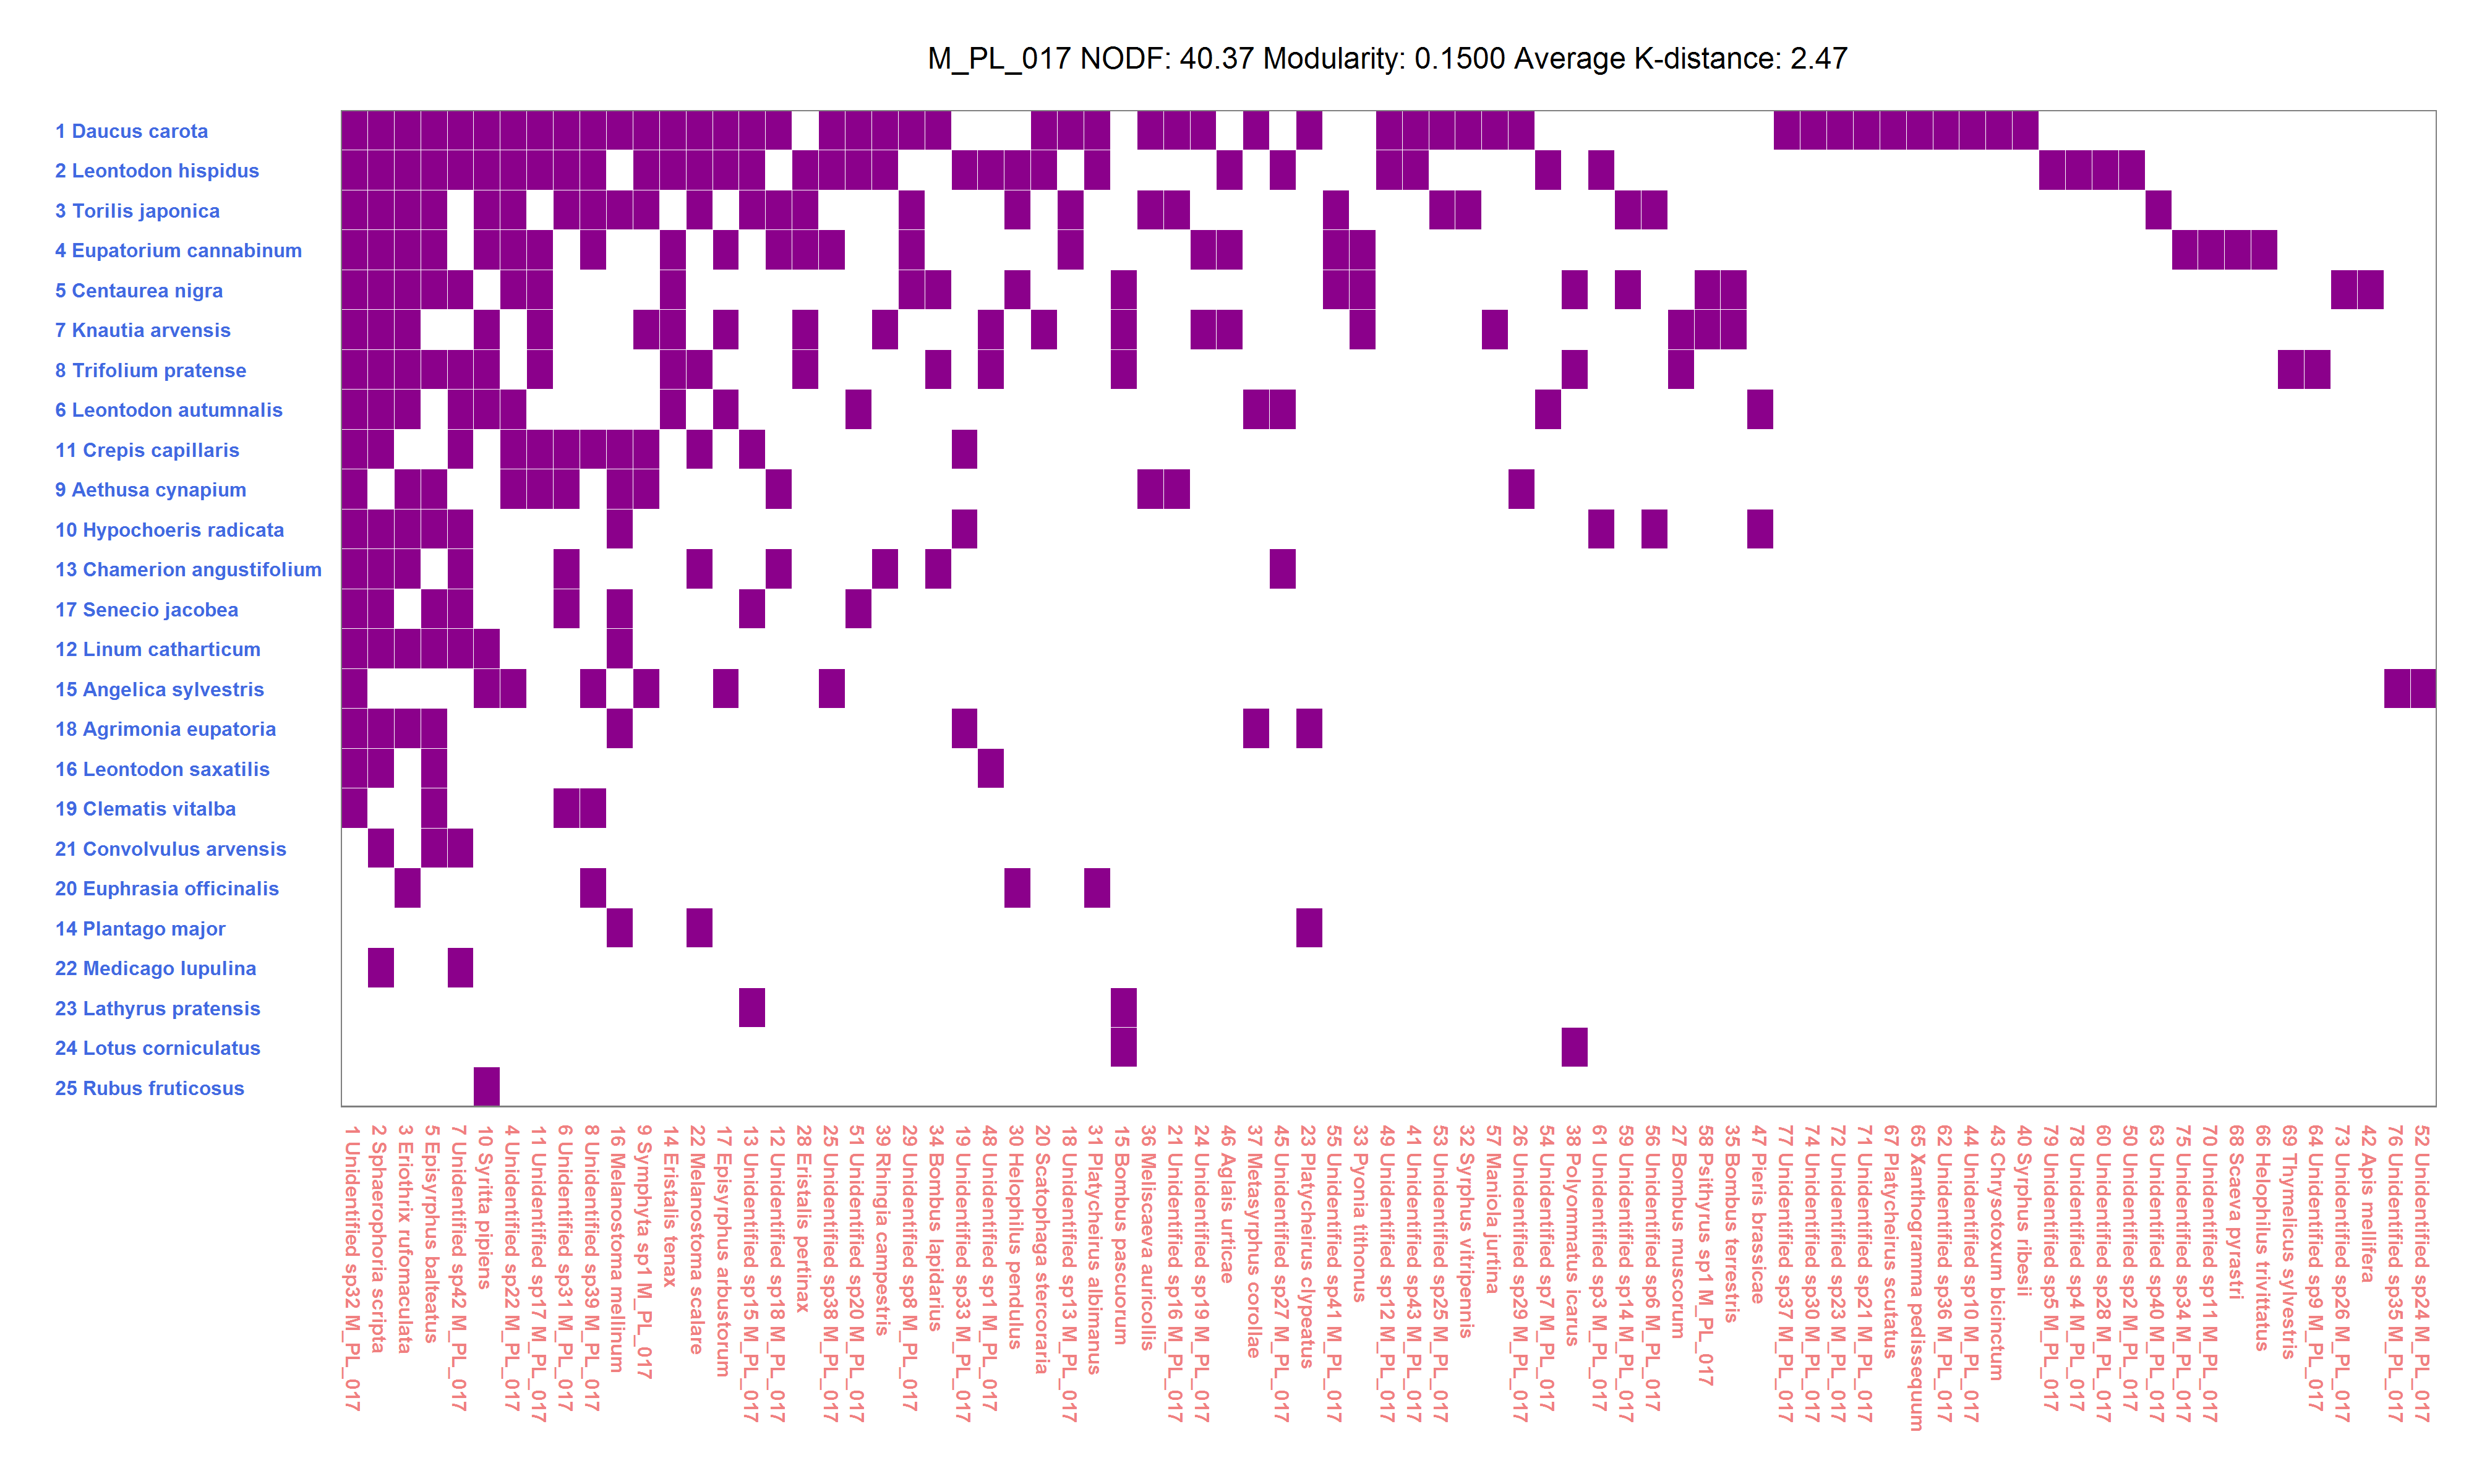
\includegraphics[scale=0.33]{Figures/VIS_M_PL_017_matrix.png}
\caption{Matriz de adyacencia de una red de polinizadores en Bristol, Inglaterra \cite{memmott1999structure}.}
\label{fig:VIS_matrix_PL_001}
\end{figure}

Una alternativa que algunos autores han explorado es utilizar representaciones convencionales para redes no bipartitas, asignando un color o forma específicos para cada clase \cite{mello2011missing,genini2010cheaters,toju2014assembly}. Esta solución tiene la ventaja de que se percibe mucho mejor la red y las relaciones indirectas que hemos mencionado. El precio que se paga es que los diagramas se vuelven muy complicados de entender con redes de tamaño medio (figura \ref{fig:VIS_grafos_weboflife}).

\begin{figure}[h!]
\centering
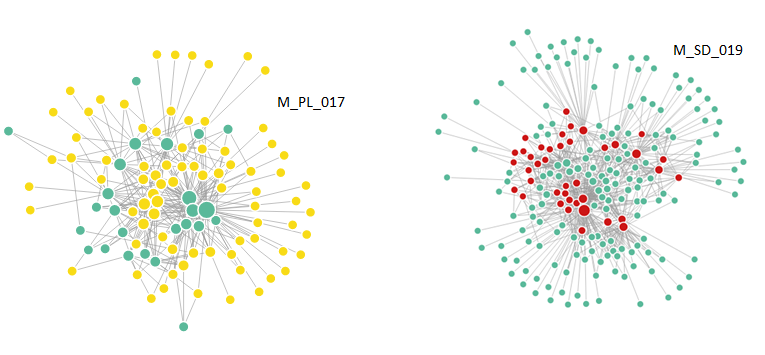
\includegraphics[scale=0.66]{Figures/VIS_grafos_weboflife.png}
\caption{Representación de dos redes de la colección \textit{web of  life} mediante la herramienta de visualización que ofrece la página web.}
\label{fig:VIS_grafos_weboflife}
\end{figure}

\clearpage
\section{Objetivos}

En esta tesis desarrollaremos aportaciones teóricas y computacionales al modelado del mutualismo en ecología con las siguientes metas:

\begin{enumerate}
\item Construir modelos dinámicos alternativos que eviten las limitaciones conocidas de los actuales.
   \begin{enumerate}
		\item Deben limitar las poblaciones bajo cualquier circunstancia.
		\item Evitarán los problemas derivados de la formulación de Pearl.
		\item Permitirán una explicación biológica de sus propiedades analíticas.
   \end{enumerate}
   
\item Describir las propiedades estructurales de las redes mutualistas basada únicamente en su topología.
		\begin{enumerate}
		\item Las magnitudes deberán explicar las propiedades del mutualismo tanto a escala local como a escala global.
		\item Se establecerá la relación de las citadas propiedades topológicas con los índices más habituales en la descripción de las redes mutualistas.
		\end{enumerate}
		
\item Construir nuevos tipos de visualización que superen las limitaciones del diagrama bipartito y de la matriz de interacción para el tamaño habitual de las redes reales.

\item Estudiar la resistencia de las redes mutualistas y las posibles políticas de conservación a la luz de su caracterización topológica.
\begin{enumerate}
		\item Comparar los criterios de ordenación existentes con los que surjan del desarrollo de la tesis.
		\item Validar los resultados con un conjunto amplio de redes reales.
		\end{enumerate}
		
\item Publicar en modalidad \textit{Open Source} todo el software desarrollado con dos propósitos.
 \begin{enumerate}
		\item Reproducibilidad de los resultados obtenidos para su validación, crítica o refutación por otros investigadores.
		\item Poner en manos de la comunidad científica las herramientas que permitan aprovechar los resultados teóricos de este trabajo.
		\end{enumerate}
\end{enumerate}


\section{Estructura de la tesis}

La tesis se divide en cinco capítulos además de este de introducción. En el capítulo \ref{chapterDINAMICA} se exponen dos modelos dinámicos alternativos al más utilizado en la literatura reciente, el denominado \textit{tipo II}. El primero funciona con capacidad de carga (\textit{carrying capacity}) constante. El segundo, con saturación del beneficio mutualista.

El capítulo \ref{chapterESTATICA} es un análisis de la estructura de las redes mutualistas que emplea una técnica clásica de teoría de grafos, la \textit{descomposición k-core}. Esta herramienta permite definir medidas locales y globales de centralidad de las especies, basándose exclusivamente en propiedades topológicas.

Las visualizaciones de redes mutualistas habituales no funcionan bien a partir de unas pocas decenas de especies. Las \textit{k-magnitudes} definidas  en el capítulo \ref{chapterESTATICA} son la base para la construcción de los nuevos tipos de gráfico que hemos desarrollado, tal y como se explica en el capítulo \ref{chapterVISUALIZACIONES}.

En el capítulo \ref{ChapterDESTRUCCION} se realiza un estudio estático de la resistencia de las redes mutualistas. En él se comparan los índices de ordenación más populares con los que surgen de la \textit{k-estructura} de las redes.

En el capítulo \ref{chapterCONCLUSIONES} se elaboran las conclusiones de la tesis.

Cierran la memoria los manuales de usuario de las dos aplicaciones desarrolladas.